\chapter{Progress}\label{progress}
\section{Rheology and Sliding Study}\label{study1}
Building upon the diagnostic ISMIP-HOM experiments in~\cite{Pattyn_2008}, I extend the prognostic experiment F to systematically investigate the combined effects of rheology and basal sliding within this benchmark ice sheet model. The original experiment F included two scenarios: One with a frozen bed (no-slip) and another with linear sliding.
My study expands upon these conditions by also incorporating non-linear rheology. This addition generates four distinct scenarios for comparison:
\begin{itemize}
\item{\bf{S1}:} No-slip (frozen) bed + Linear rheology ($n=1$).
\item{\bf{S2}:} No-slip (frozen) bed + Non-linear rheology ($n=4$).
\item{\bf{S3}:} Linear sliding + Linear rheology ($n=1$).
\item{\bf{S4}:} Linear sliding + Non-linear rheology ($n=4$).
\end{itemize}
The method I follow to ensure that different model rheologies start from identical initial conditions is based on the re-scaling method by Getraer and Morlighem (2025)~\cite{Getraer_2025}. Their formula ensures that the initial ice viscosity—and therefore strain rates for a given stress—is identical between simulations with different rheologies.
For the non-linear scenarios I am considering $n = 4$, since the assumption of $n = 3$ for ice deformation is not universally supported and values of $n > 3$ have been inferred from real‐world glaciers.
\begin{figure}[H]
    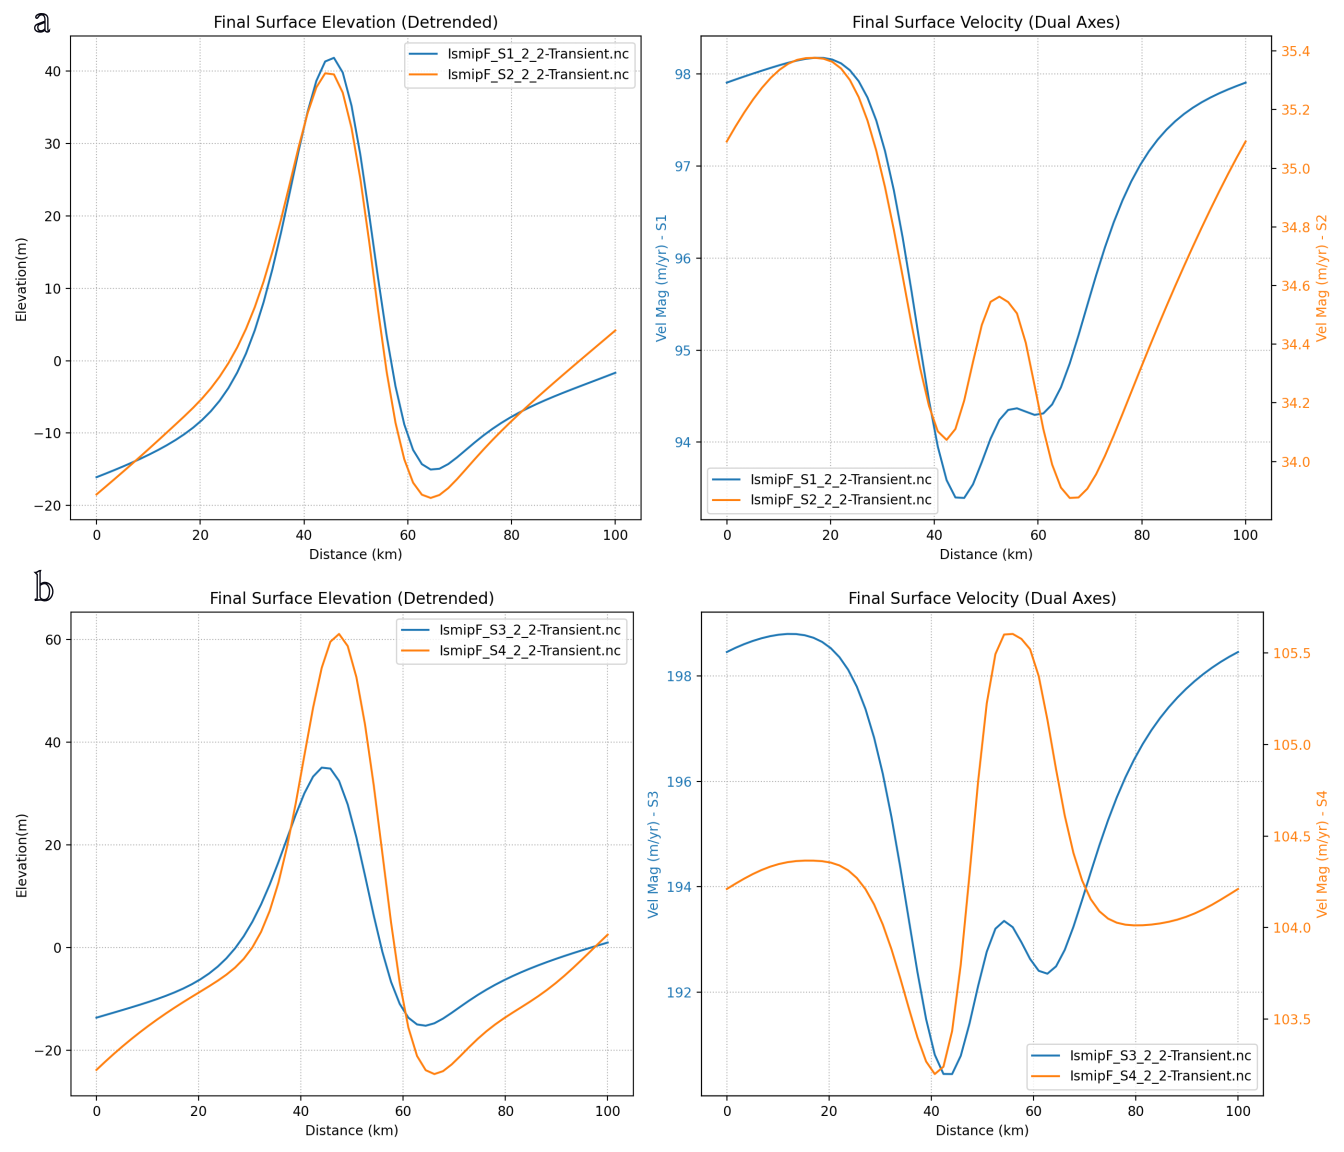
\includegraphics[scale=0.40]{figures/combined_elevation_detrended_surface_velocity_['S1']_['S2']_['S3']_['S4'].png}
    \caption{(a) Final surface elevations and velocities for the original frozen bed Experiment F (S1) and the corresponding transformed to non-linear rheology experiment (S2) (b) Final surface elevations and velocities for the original sliding bed Experiment F (S3) and the corresponding transformed to non-linear rheology experiment (S4).}
    \label{fig:elev_vel_S1_S2_S3_S4}
\end{figure}

The linear results depicted in blue in Figure~\ref{fig:elev_vel_S1_S2_S3_S4} are consistent with the surface elevation and velocities found for Experiment F in~\cite{Pattyn_2008}. Meanwhile, the non-linear scenarios (S2 and S4) shown in orange  represent the first key finding of this analysis. The marked differences in both final surface elevation and velocity compared to the linear counterparts (S1, S3) provide crucial evidence for my first research question (``How does the bed topography manifest on the ice surface?''). Using $n = 4$ leads to a strong non-linear relationship where a small increase in stress yields a much larger increase in deformation. The results demonstrate that the choice of rheology is an important control on the bed-to-surface signal transfer. Implying that a succesful inversion framework like BedSAT must account for non-linear effects.

\section{Data Processing, Visualization and Analysis Tools}\label{analysis_tools}
This study is supported by a suite of interconnected scripts and tools designed for generating conditions, running simulations, processing output, and performing scientific analysis.
The core of this study is a time evolution flow simulation of fully grounded ice over 300 years with daily time steps. This simulation is designed to systematically investigate the relationship between basal geometry, ice rheology and flow response by running a series of ISMIP-HOM style experiments~\cite{Pattyn_2008} that can later be analysed in detail with other data processing tools.
\begin{figure}[H]
    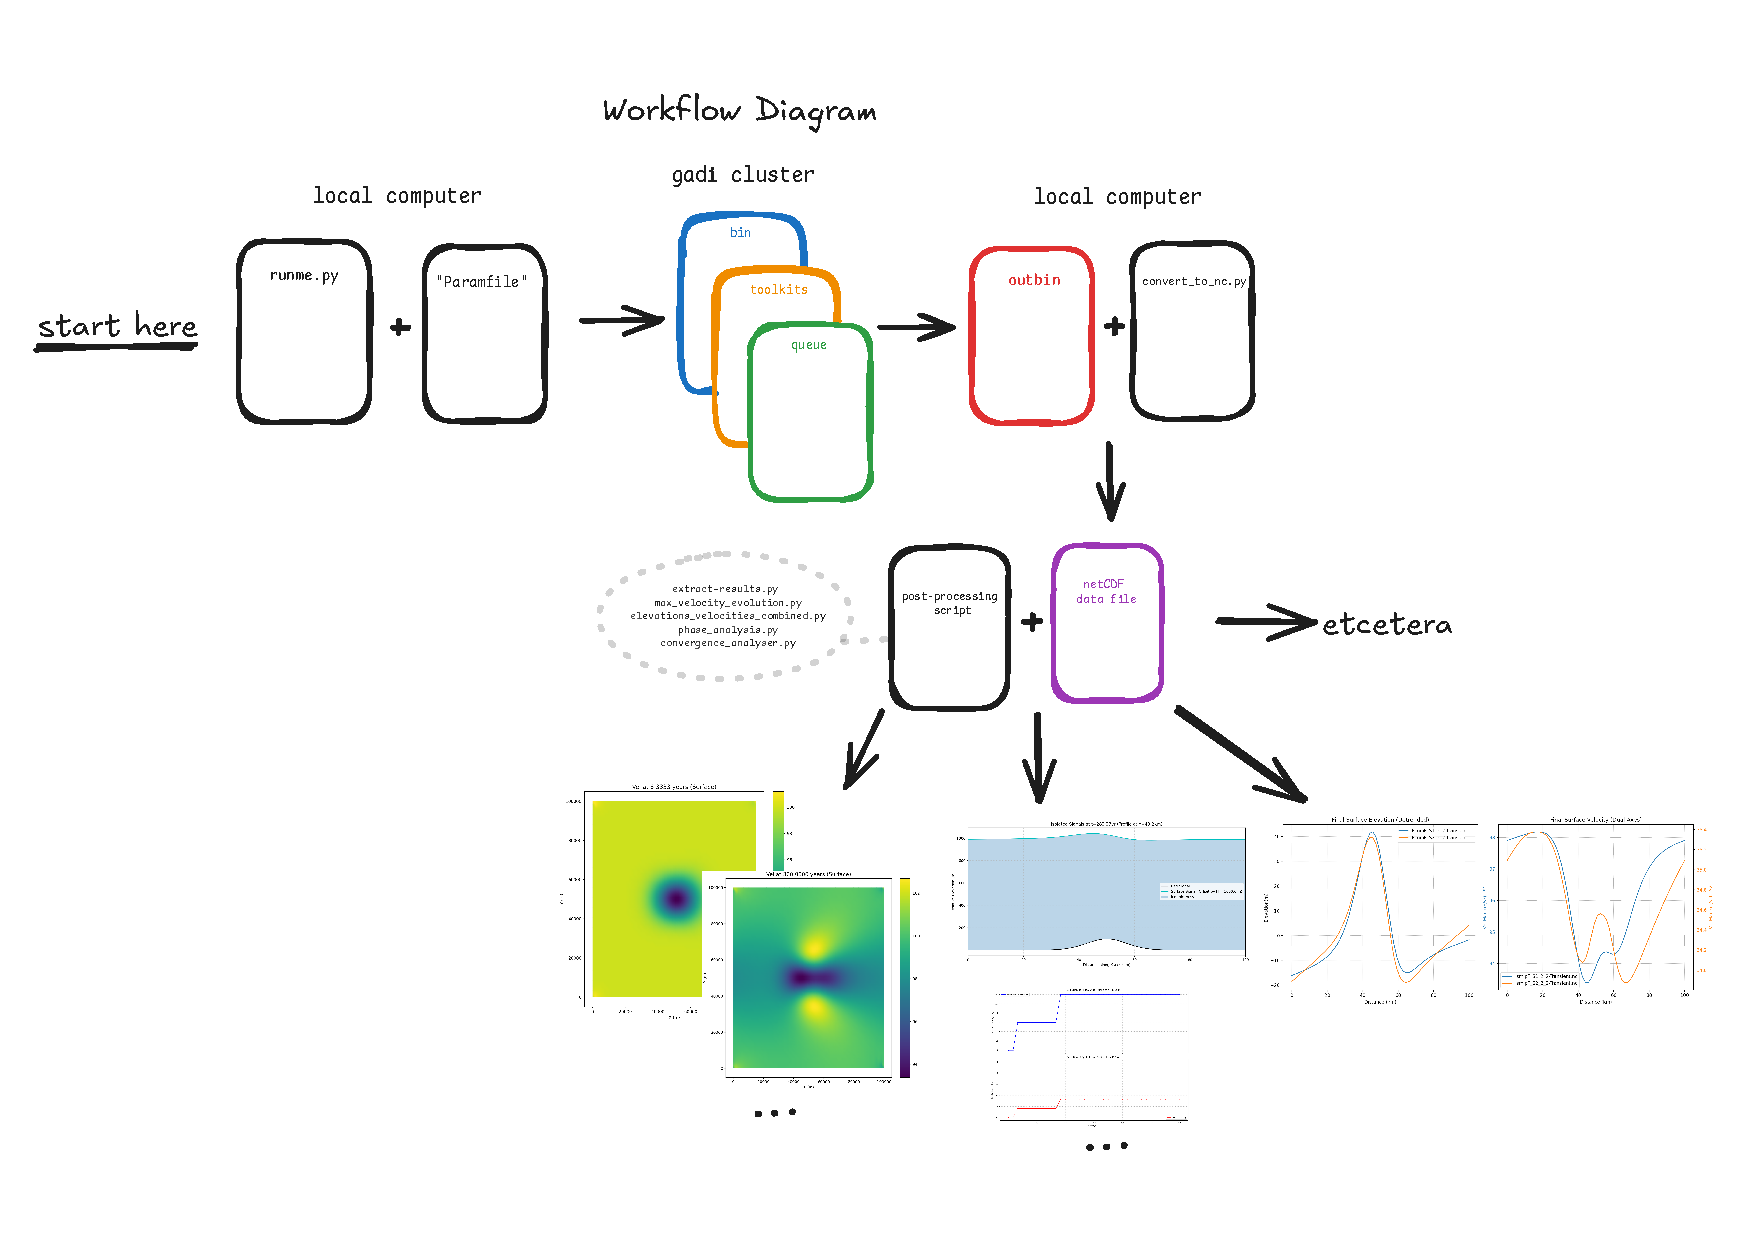
\includegraphics[scale=0.55]{figures/workflow_diagram.pdf}
    \caption{Diagrammatic representation of the current workflow using my ice simulation and analysis suite. For a particular simulation I will extract the results and visually inspect the output using  all analysis scripts in the suite.}\label{fig:workflow}
\end{figure}
\begin{enumerate}
\item{Binary to NetCDF Conversion}: Converts ISSM \texttt{.outbin} files into the standard, portable NetCDF format.
\item{Result Extraction and Visualization}: Automatically finds and processes NetCDF files to generate visualisations of key fields like velocity and pressure. 
\item{Targeted Scientific Plotting}: Additional scripts are used to create specific scientific plots.
\end{enumerate}
\begin{figure}[H]
    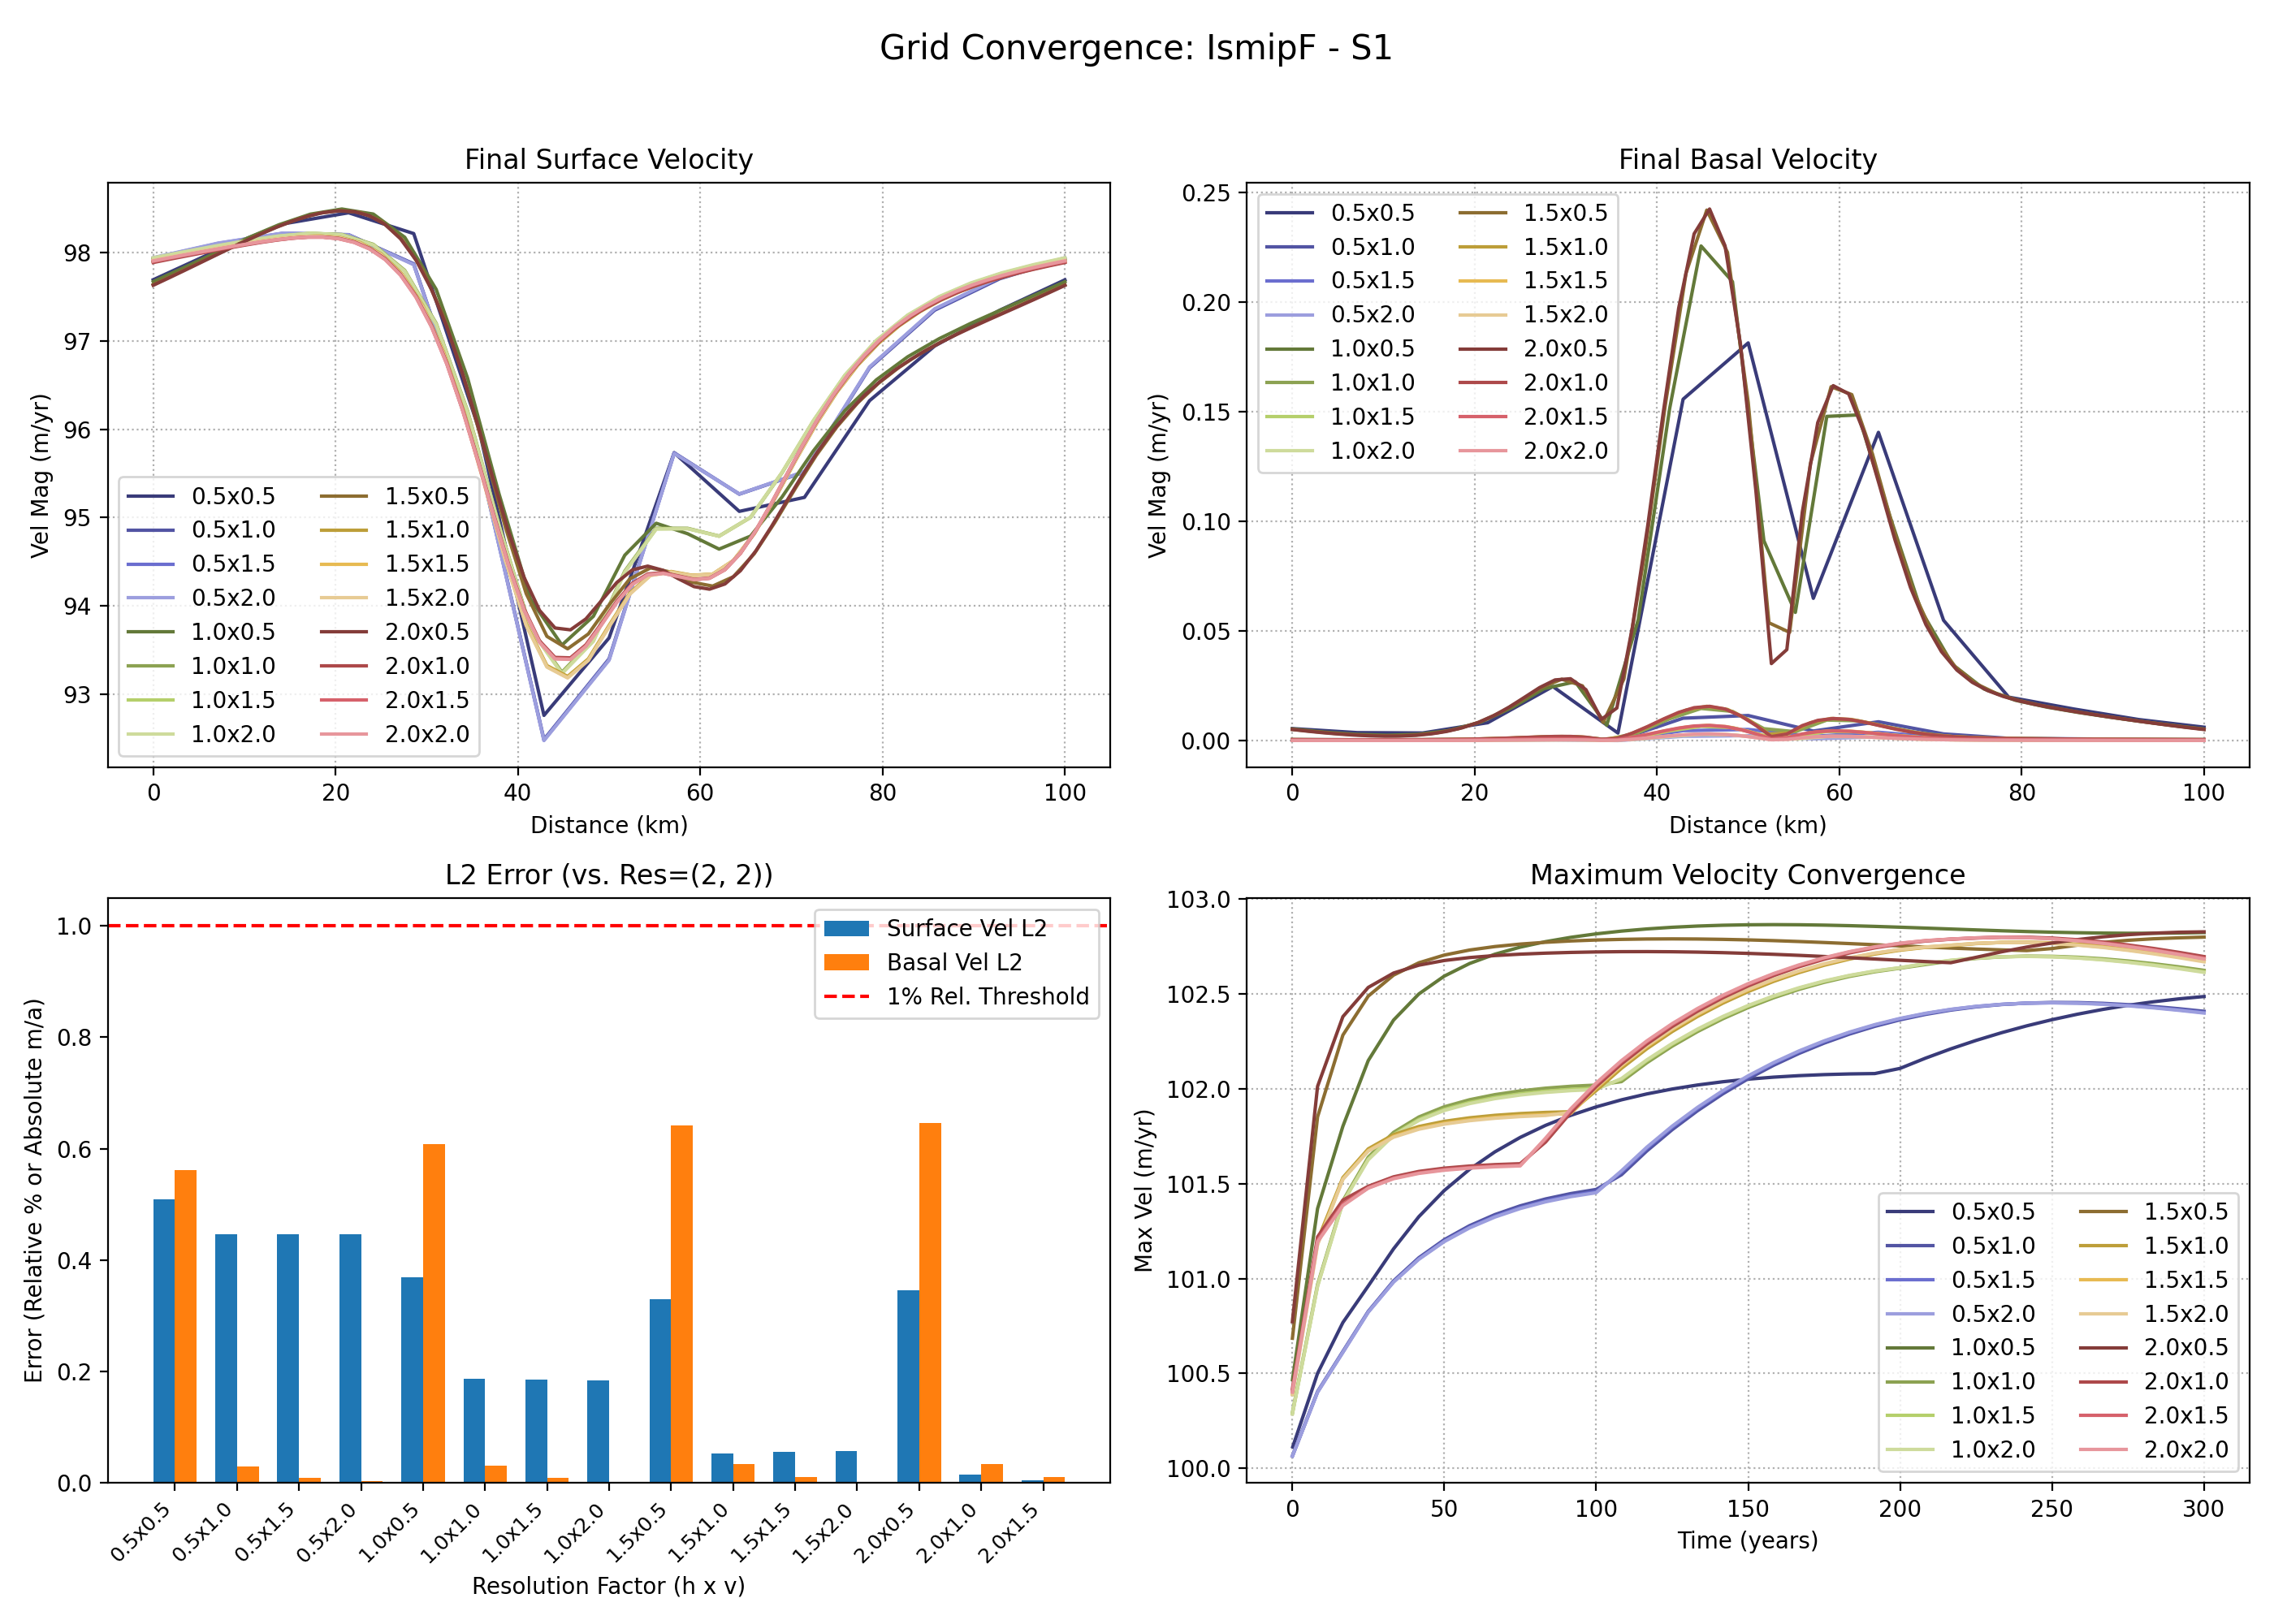
\includegraphics[scale=0.40]{figures/IsmipF_S1_convergence_summary.png}
    \caption{Grid convergence analysis for Scenario S1 (frozen bed, linear rheology, $n=1$). The four panels show: (top-left) final surface velocity profiles and (top-right) final basal velocity profiles for 16 different mesh resolutions; (bottom-left) the L2 relative error of each simulation compared to the highest-resolution mesh ($2.0\times2.0$), with a 1\% relative error threshold indicated by the dashed line; and (bottom-right) the evolution of the maximum velocity over the 300-year simulation period}
    \label{fig:grid_conv_S1}
\end{figure}
\begin{figure}[H]
    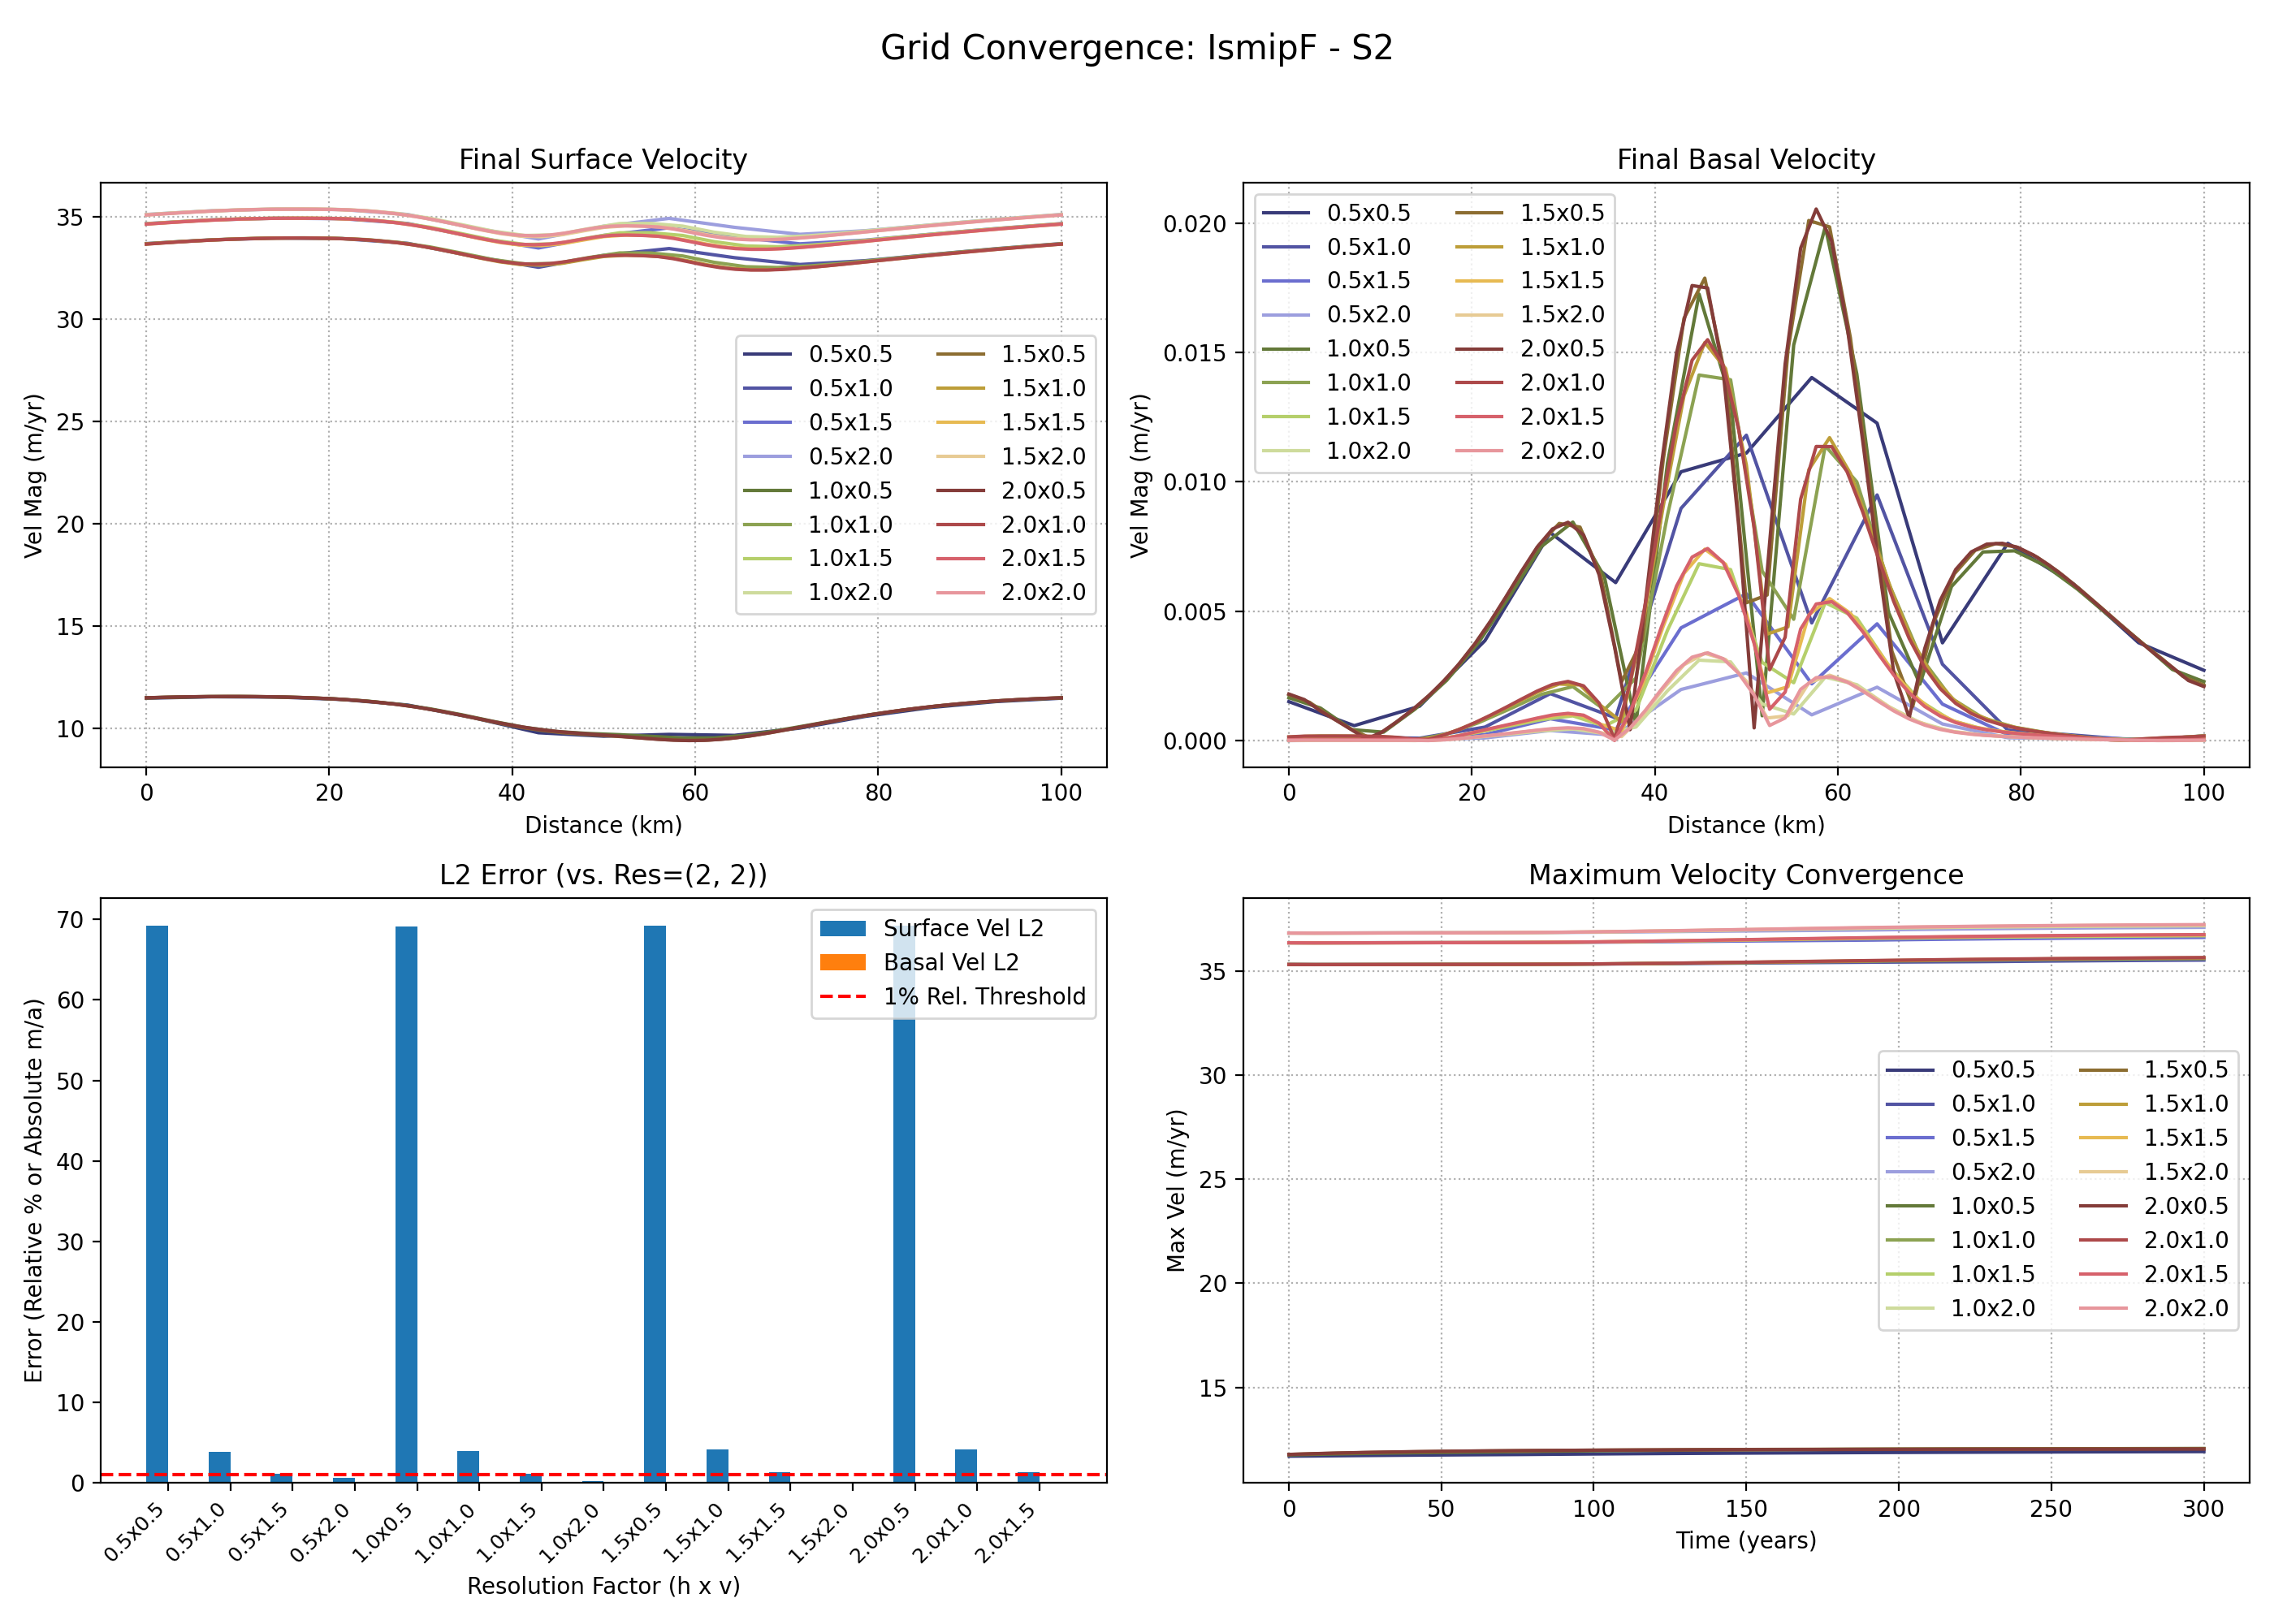
\includegraphics[scale=0.40]{figures/IsmipF_S2_convergence_summary.png}
    \caption{Grid convergence analysis for Scenario S2 (frozen bed, non-linear rheology, $n=4$). An extension of ISMIP-HOM Experiment F. The panels display the same metrics as Figure~\ref{fig:grid_conv_S1}. This scenario exhibits high sensitivity to vertical resolution refinement, with low-resolution simulations showing the highest errors and converging to a much slower flow state ($\approx~11$ m/a) compared to high-resolution runs ($\approx~37$ m/a).}
    \label{fig:grid_conv_S2}
\end{figure}
\begin{figure}[H]
    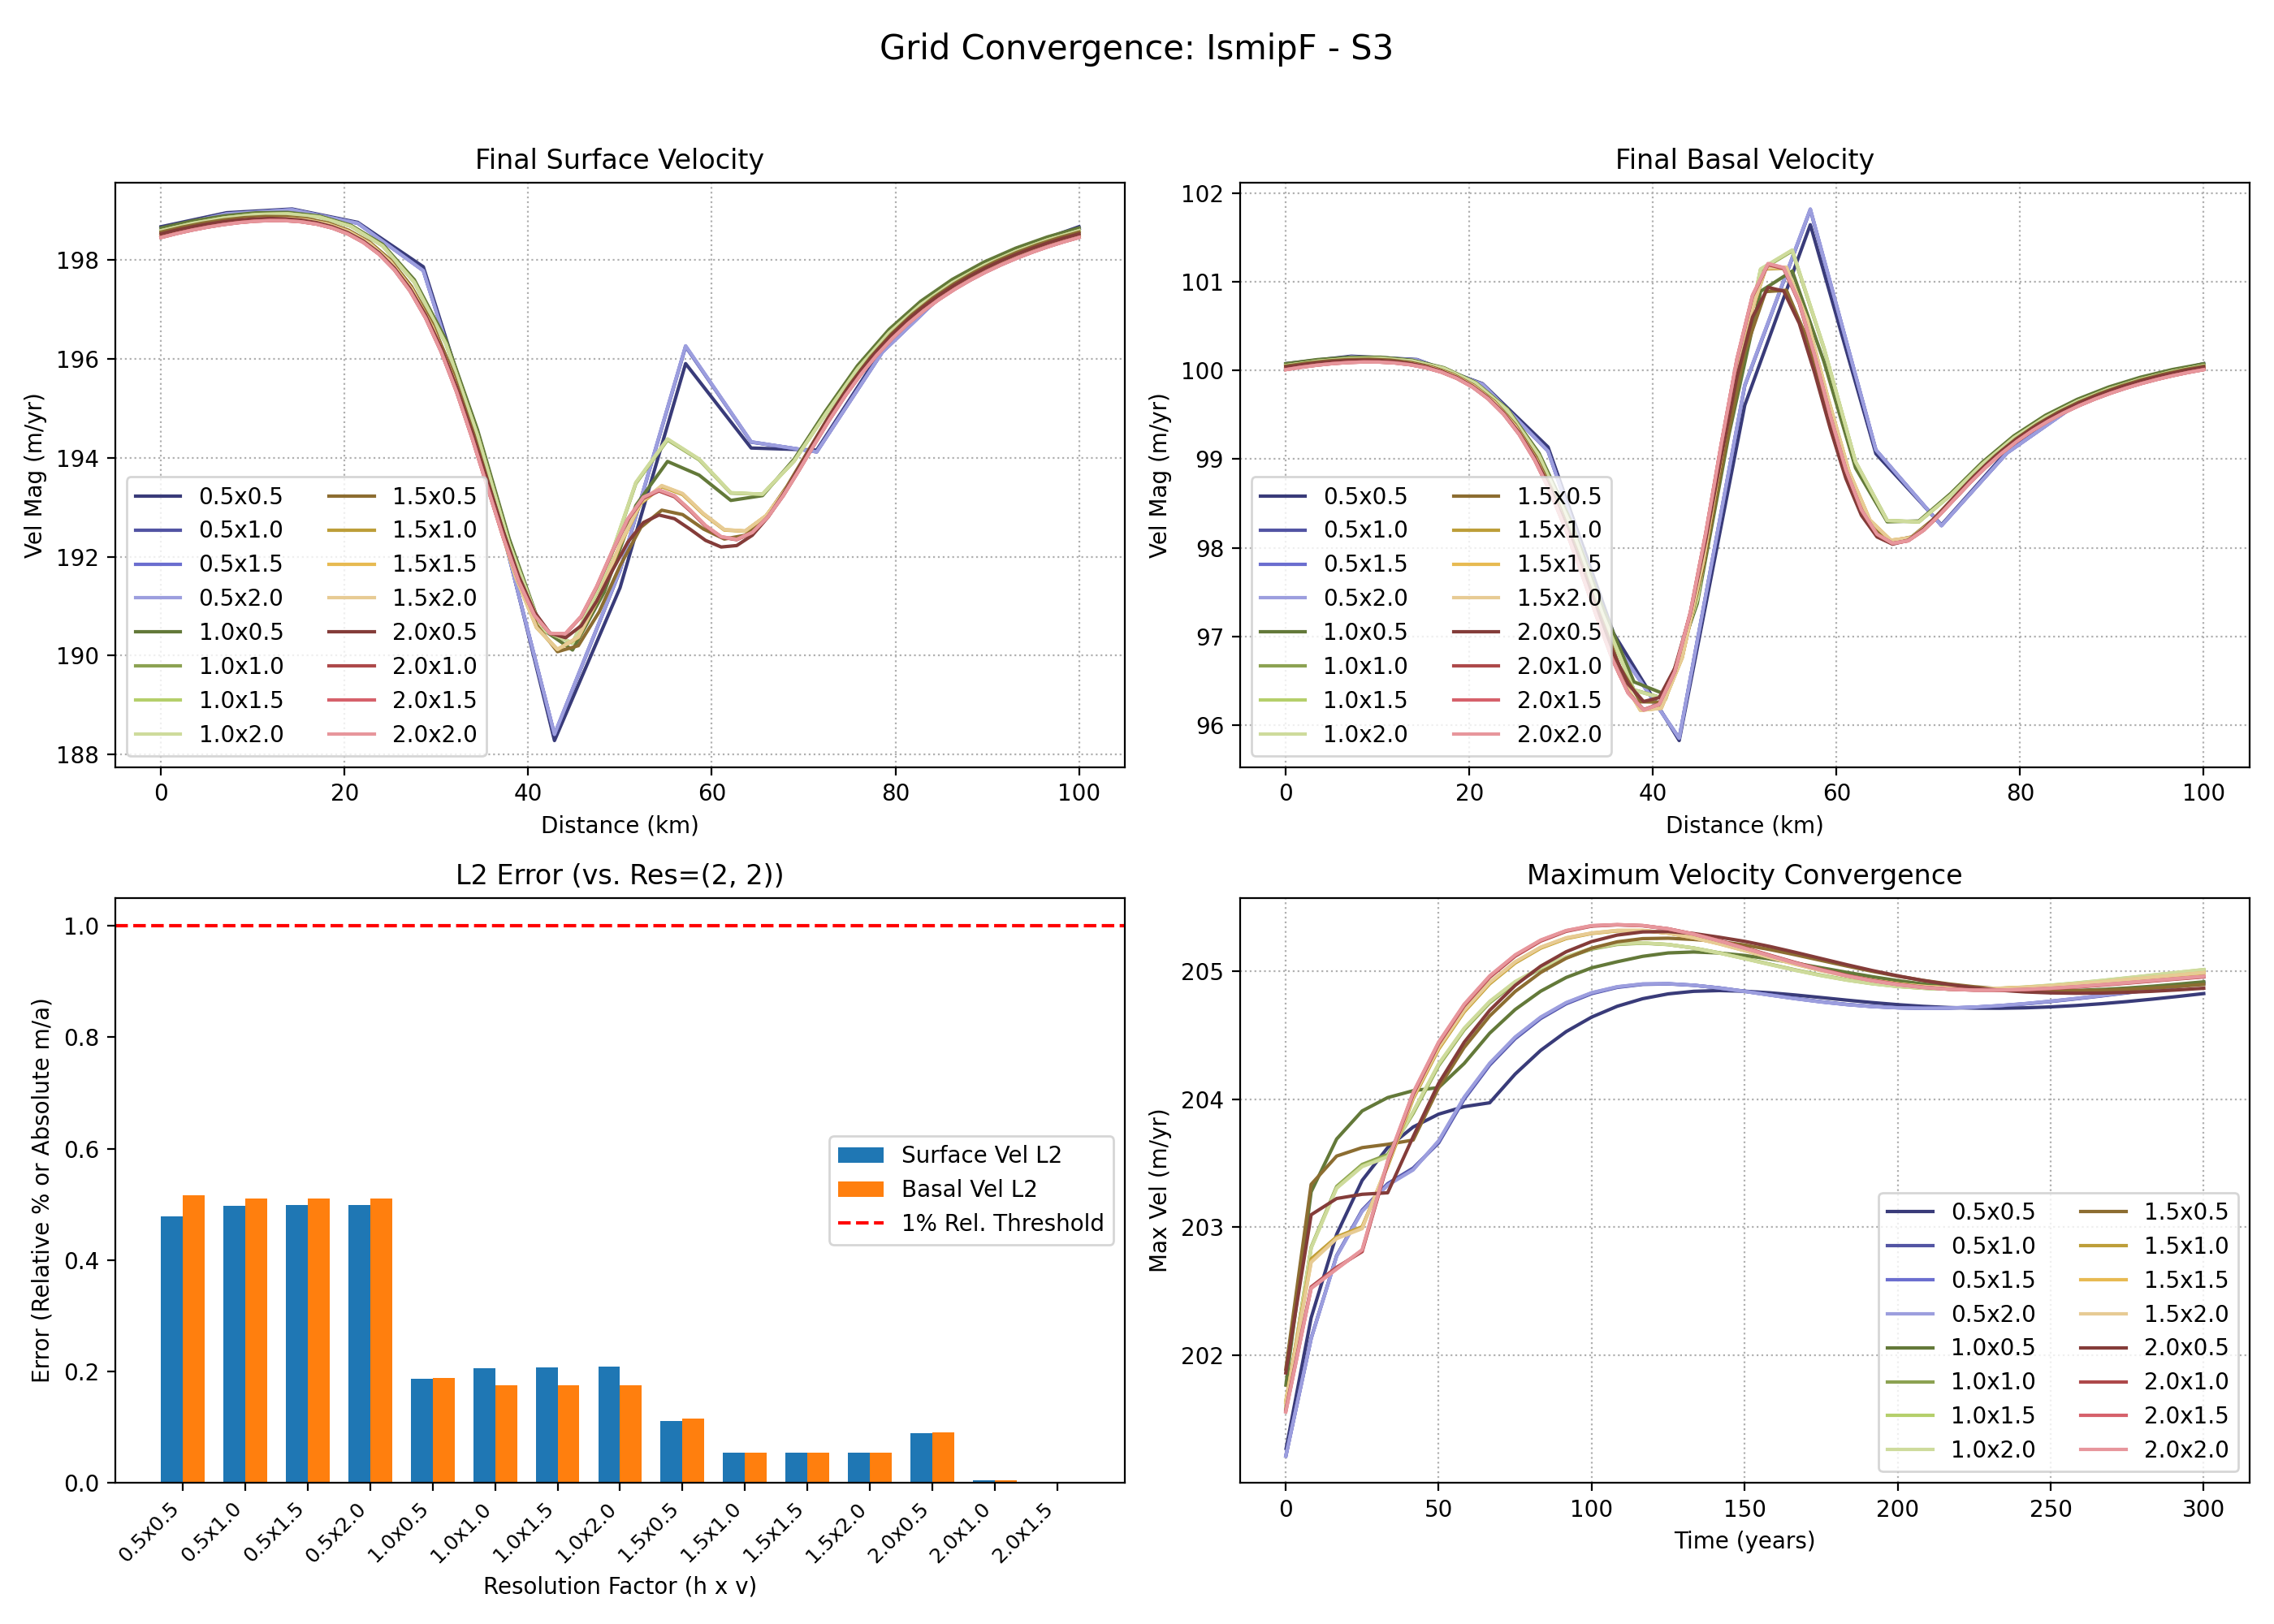
\includegraphics[scale=0.40]{figures/IsmipF_S3_convergence_summary.png}
    \caption{Grid convergence analysis for Scenario S3 (linear sliding, linear rheology, $n=1$). The four panels show: (top-left) final surface velocity profiles and (top-right) final basal velocity profiles for 16 different mesh resolutions; (bottom-left) the L2 relative error of each simulation compared to the highest-resolution mesh ($2.0\times2.0$), with a 1\% relative error threshold indicated by the dashed line; and (bottom-right) the evolution of the maximum velocity over the 300-year simulation period}
    \label{fig:grid_conv_S3}
\end{figure}
\begin{figure}[H]
    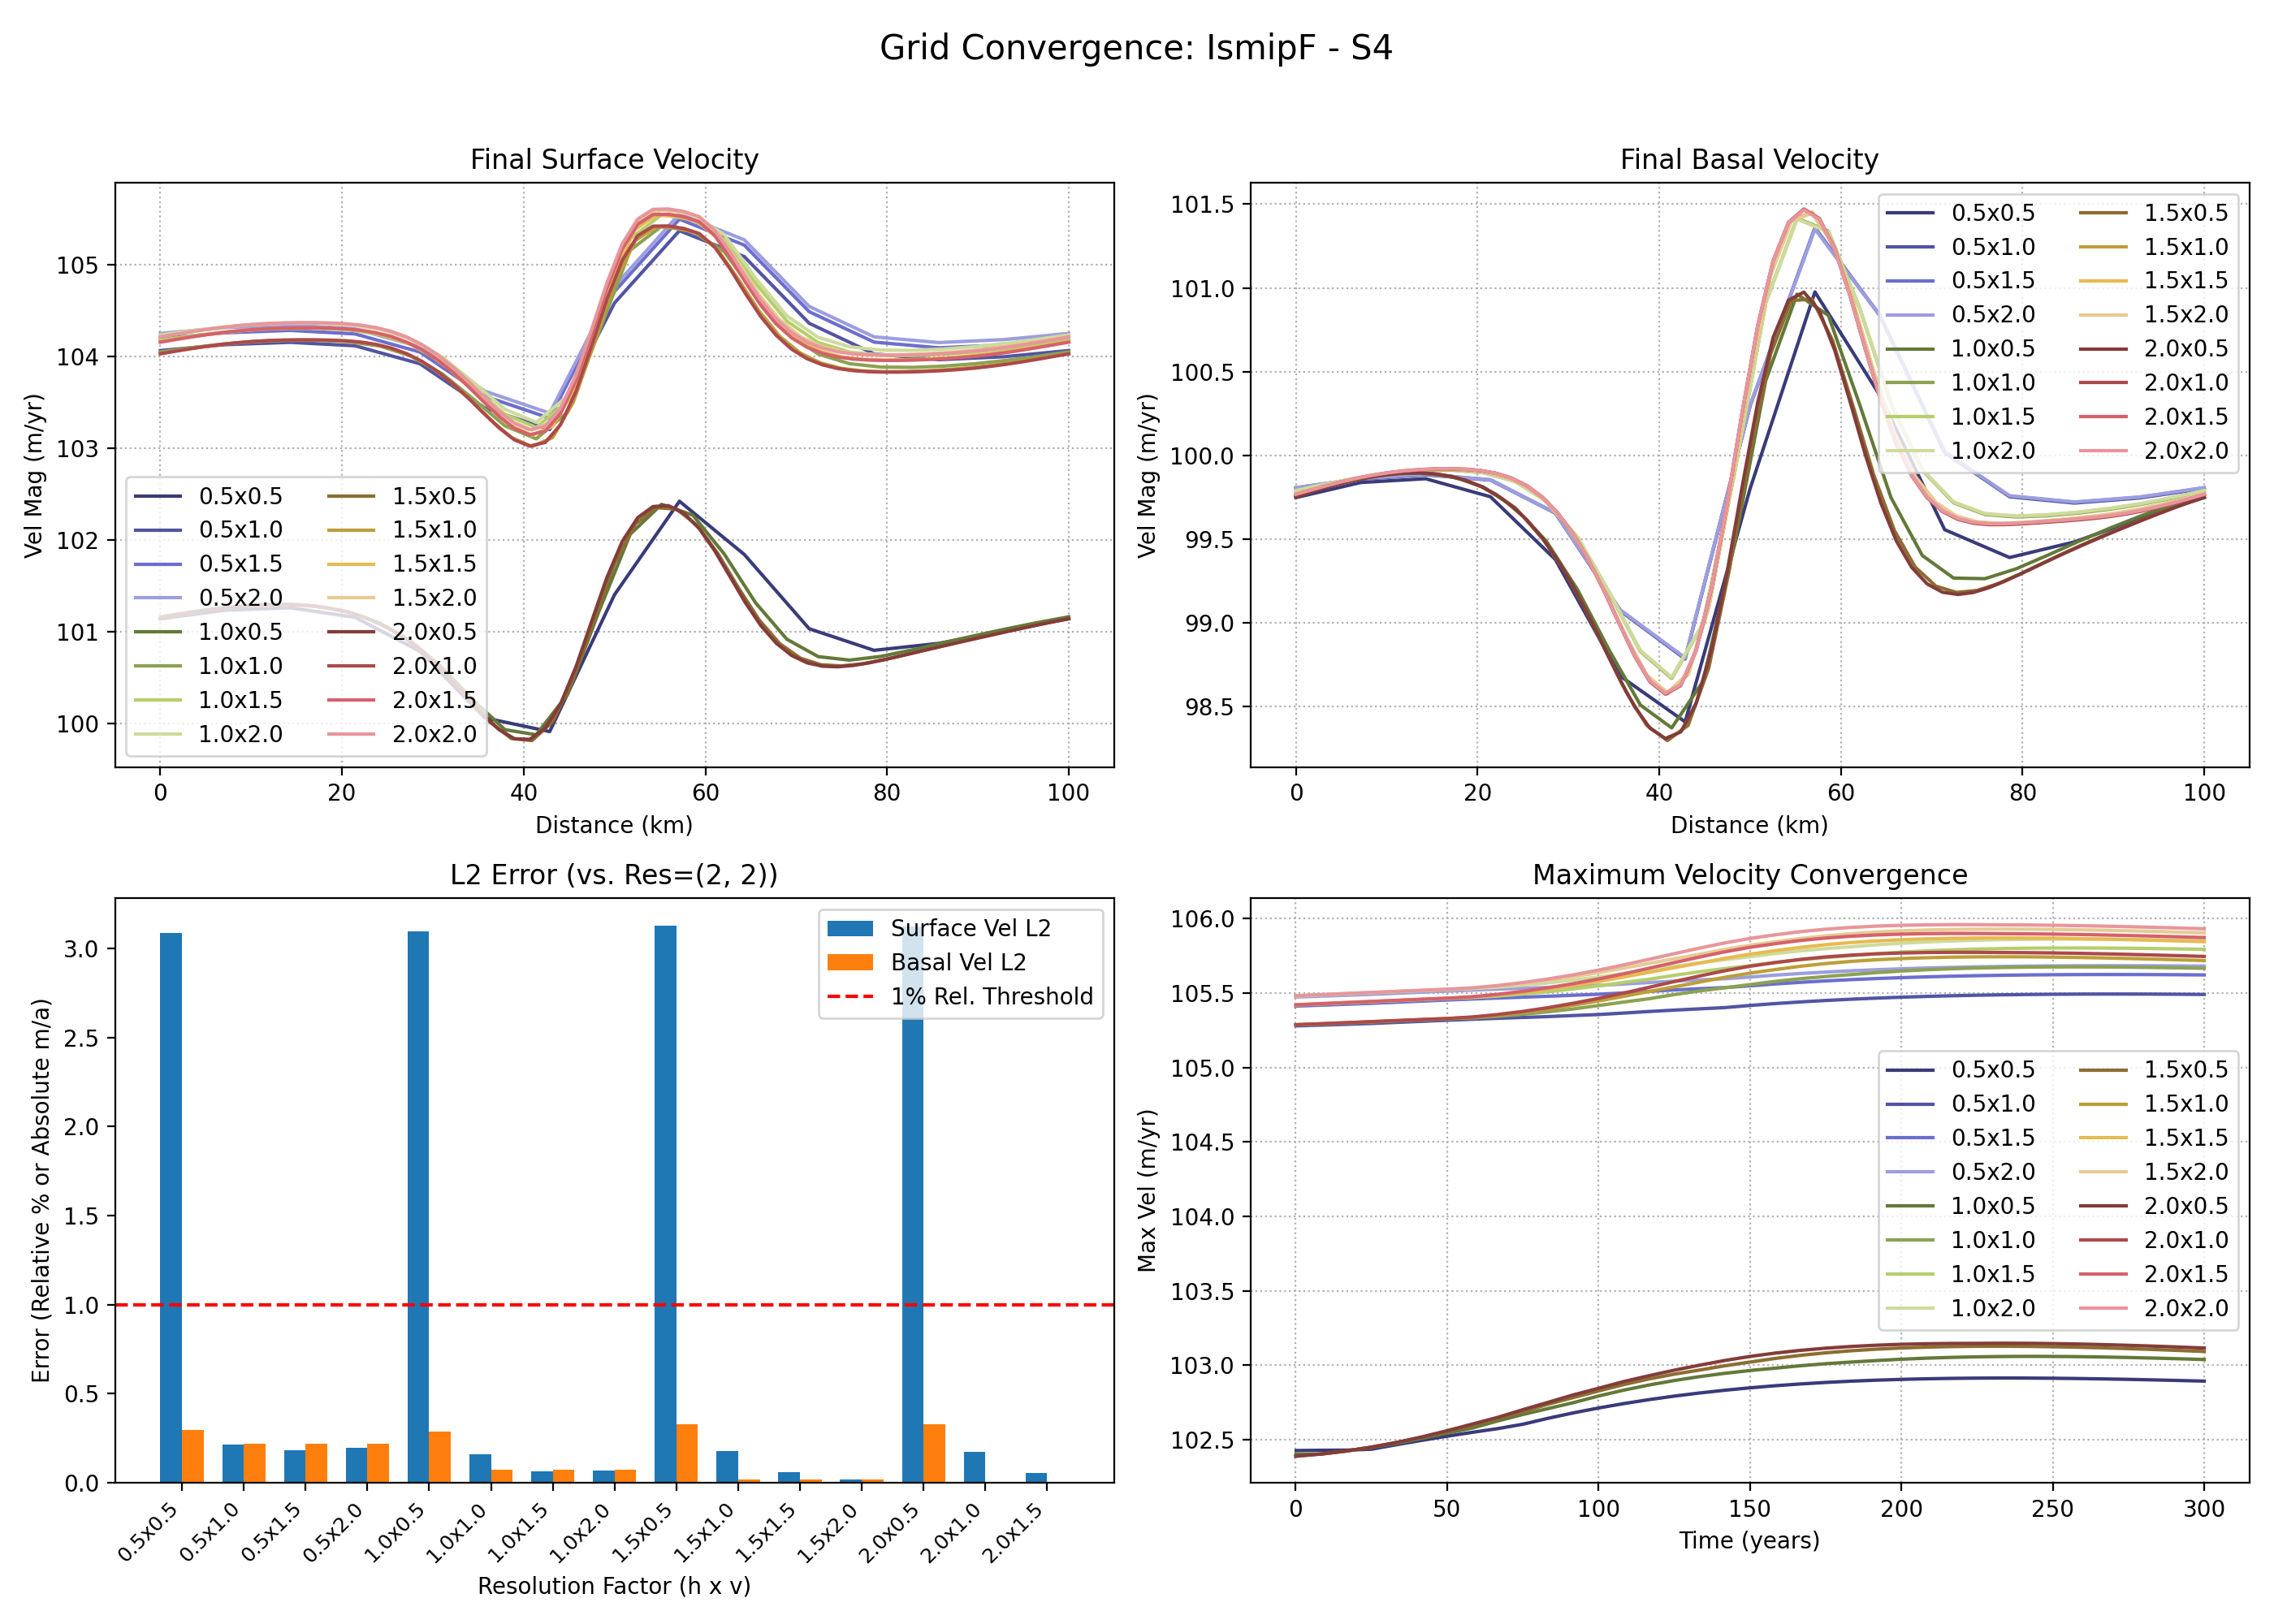
\includegraphics[scale=0.40]{figures/IsmipF_S4_convergence_summary.png}
    \caption{Grid convergence analysis for Scenario S4 (linear sliding, non-linear rheology, $n=4$). Another extension of ISMIP-HOM Experiment F, similarly to the other non-linear case (S2) in Figure~\ref{fig:grid_conv_S2}, this scenario is highly sensitive to vertical resolution.  The convergence analysis shows that the 1\% relative error threshold is only achieved for simulations using the highest vertical resolution factor (2.0)}
    \label{fig:grid_conv_S4}
\end{figure}
Convergence analyses show the simulations as most sensitive to vertical resolution. Particularly, non-linear rheology scenarios in Figures~\ref{fig:grid_conv_S2} and~\ref{fig:grid_conv_S4}, where refining vertical resolution produces qualitatively different results. The convergence threshold of 1\% is only achieved for both S2 and S4 with the finest resolution. 
The next phase of my research involves a suite of realistic synthetic bedrock topographies—closely mimicking the conditions found in Antarctica—in order to further inform the development of BedSAT.